\documentclass[a4paper,12pt]{article}

% \usepackage[french]{babel}


\usepackage[utf8]{inputenc}
\usepackage[T1]{fontenc}
\usepackage{amssymb,amsthm,amsmath,amsfonts}
\usepackage{textcomp}
%\usepackage{bbm}

\usepackage{framed}

\def\BF{\begin{framed} }
\def\EF{\end{framed} }

\frenchspacing

\long\def\/*#1*/{}

\def\gal{\text{Gal}}

\setlength{\textwidth}{15cm}
\setlength{\hoffset}{0.46cm}
\setlength{\oddsidemargin}{0cm}
\setlength{\marginparsep}{0cm}
\setlength{\marginparwidth}{0cm}
\setlength{\textheight}{24.2cm}
\setlength{\headheight}{0cm}
\setlength{\topmargin}{0cm}
\setlength{\headsep}{0cm}
\setlength{\paperwidth}{29cm}


\frenchspacing

\long\def\/*#1*/{}

\def\gal{\text{Gal}}

% \setlength{\textwidth}{15cm}
% \setlength{\hoffset}{0.46cm}
% \setlength{\oddsidemargin}{0cm}
% \setlength{\marginparsep}{0cm}
% \setlength{\marginparwidth}{0cm}
% \setlength{\textheight}{24.2cm}
% \setlength{\headheight}{0cm}
% \setlength{\topmargin}{0cm}
% \setlength{\headsep}{0cm}
% \setlength{\paperwidth}{29cm}

\def\RR{\mathbb{R}}
\def\CC{\mathbb{C}}
\def\NN{\mathbb{N}}
\def\ZZ{\mathbb{Z}}
\def\Q{\mathbb{Q}}
\def\F{\mathbb{F}}
\def\1{\mathbbm{1}}

% Usual sets of numbers  
\def\bA{{\Bbb A}}
\def\bC{{\Bbb C}}
\def\bF{{\Bbb F}}
\def\bK{{\Bbb K}}
\def\bN{{\Bbb N}}
\def\bP{{\Bbb P}}
\def\bQ{{\Bbb Q}}
\def\bR{{\Bbb R}}
\def\bZ{{\Bbb Z}}


\DeclareMathOperator{\pgcd}{pgcd}
\DeclareMathOperator{\ppcm}{ppcm}
\DeclareMathOperator{\GL}{GL}
\DeclareMathOperator{\Aut}{Aut}
\DeclareMathOperator{\Inn}{Inn}
\DeclareMathOperator{\id}{id}
\DeclareMathOperator{\End}{End}
\DeclareMathOperator{\Hom}{Hom}

\newcommand{\FF}{\mathbb{F}_q}

\def\ggauche{\textgravedbl}
\def\gdroite{\textacutedbl}


% Usual sets of numbers  
\def\bA{{\Bbb A}}
\def\bC{{\Bbb C}}
%\def{\bF{\Bbb F}}
\def\bK{{\Bbb K}}
\def\bN{{\Bbb N}}
\def\bP{{\Bbb P}}
\def\bQ{{\Bbb Q}}
\def\bR{{\Bbb R}}
\def\bZ{{\Bbb Z}}

\def\gc{\hbox{\goth c}}
\def\sevengc{\hbox{\sevengoth c}}
\def\mathfrak{\hbox{\goth S}}
\def\tr{\mathop{\rm tr}}
\def\Gal{\mathop{\rm Gal}}
\def\syquad#1#2{\left({#1\over #2}\right)}


\reversemarginpar

\newcommand{\dual}{\vee}

\newtheorem{enonce}{Exercice}
\newenvironment{E}[0]{\begin{enonce}\rm}{\bigskip \end{enonce}}

\begin{document}

\begin{center}
\textbf{CC3 - 2025} \hfill \textbf{Durée :  90m} \\
\vspace{1em}
{\Large Calcul intégral, introduction aux probabilités}

\vspace{1em}

\end{center}


Aucun document ni matériel électronique n’est autorisé. Les exercices sont indépendants mais chaque exercice a sa propre cohérence. La qualité de la rédaction sera grandement prise en
compte dans la notation.

\bigskip

\hline
\vspace{1em}

\noindent
\textbf{Exercice 1 : Courbes paramétrées.}

Une astroïde est une courbe plane, qui peut se définir de plusieurs
façons. En particulier, il est possible de l'obtenir en faisant
rouler un cercle de rayon $r = \frac14$ à l'intérieur d'un cercle de rayon 1. Pour cette raison, l'astroïde est une hypocycloïde de cercle à quatre points de rebroussement.

  \begin{figure}[hb]
\centering
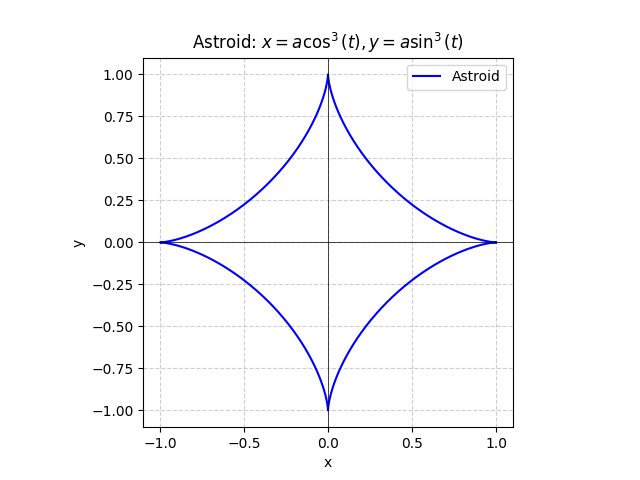
\includegraphics[scale=.7]{./asteroid.png} 
  \label{pt graphic}
\end{figure}
L'equation paramétrique de l'astroïde est donnée par :
$$ x= a\cos^3(t), y = a\sin^3(t)$$
où $a>0$ est une constante
et  $t\in[0,2\pi]$. 


\begin{enumerate}
\item
Déterminer le vecteur vitesse de la courbe paramétrée.
\item
Calculer la longueur de l'arc de cette courbe.
\end{enumerate}
\bigskip

%   \begin{figure}[hb]
% \centering
% 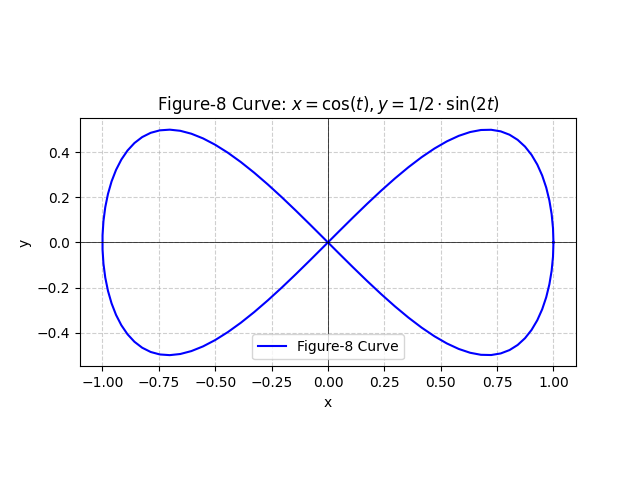
\includegraphics[scale=.7]{./fig8.png} 
% \label{lemniscate}
% \end{figure}

%   L'équation paramétrique d'une lemniscate est donnée par :
%   $$(x(t),y(t))=(\cos(t),\sin(t)\cos(t)), t \in [0,2\pi]$$
%   % $$x=\cos(t),y=a\sin(t)\cos(t), t \in [0,2\pi]$$

% \begin{enumerate}
% \item

% Déterminer le vecteur vitesse de la courbe paramétrée.

% \item 
% Calculer la longueur de l'arc pour $a=\frac12$.

% \item 
% Choisir un autre valeur de $a\neq \frac12$ et calculer la longueur de l'arc de la courbe paramétrée.

% \end{enumerate}

\hline

\bigskip

\noindent
\textbf{Exercice 2 : Intégrales doubles.}

Évaluer les intégrales doubles suivantes :  
\begin{enumerate}
\item
\[
	\iint_{A} \frac{2xy}{x^2 + y^2} \, {dx \, dy},
\]  
où 
\begin{itemize}
\item
\( A \) est la région comprise entre les cercles de rayon 1 et 2, dans le premier quadrant, c’est-à-dire :  
\[
A = \left\{ (x, y) \in \mathbb{R}^2 \ \big| \ 1 \leq \sqrt{x^2 + y^2} \leq 2,\ x \geq 0,\ y \geq 0 \right\}.
\]
\item
	$A$ est le disque de centre l'origine et de rayon 1,
	c'est-à-dire :
	$$A = \left\{ (x, y) \in \mathbb{R}^2 \ \big| x^2 + y^2 \leq 1 \right\}.$$
\end{itemize}

\item
\[
	\iint_{R} \frac{x + y}{x - y} \, {dx \, dy},
\]  
où \( R \) est la région bornée délimitée par les droites \( x - y = 1 \), \( x - y = 2 \), \( x + y = 3 \), et \( x + y = 5 \).

Utiliser un changement de variables adapté pour simplifier et calculer l'intégrale.

% \item

% \[
% 	\iint_{S} \frac{x - y}{x + y} \, {dx \, dy},
% \]  
% où \( S \) est la région dans le premier quadrant délimitée par les hyperboles \( xy = 1 \), \( xy = 4 \), et les droites \( x = y \), \( x = 2y \).

% Utilisez un changement de variables approprié pour simplifier et évaluer l'intégrale, par exemple \( u = xy \), \( v = \frac{x}{y} \), ou un autre changement pertinent.  

\end{enumerate}

% 1. Proposez un changement de variables, par exemple \( u = xy \), \( v = \frac{x}{y} \), ou un autre changement pertinent.  
% 2. Exprimez l'intégrande et la région \( R \) en fonction de \( u \) et \( v \).  
% 3. Calculez le déterminant Jacobien de la transformation.  
% 4. Transformez l'intégrale et évaluez-la sur la nouvelle région.

\hline
\bigskip

\noindent
\textbf{Exercice 3 : Probabilités conditionnelles.}

Dans une entreprise de fabrication de stylos, trois machines M1, M2 et M3 produisent respectivement 20\%, 50\% et 30\% du total des stylos. Chaque machine produit un certain pourcentage de stylos à encre bleue : M1 en produit 10\%, M2 en produit 6\% et M3 en produit 4\%.

On choisit un stylo au hasard dans la production totale, et il s'avère qu'il contient de l'encre bleue.

\begin{enumerate}
\item
Quelle est la probabilité que ce stylo ait été produit par la machine M1 ? Par M2 ? Par M3 ?
\item
Sachant qu’un stylo contient de l’encre bleue, quelle est la probabilité qu’il ait été produit par une machine qui fabrique moins de 7\% de stylos bleus ?
\end{enumerate}

\hline

\vspace{1em}


\textbf{Loi de probabilité d'une variable aléatoire discrète.}
\begin{center}
{\Large Choisir entre l'exercice 4a ou 4b.}
\end{center}
\bigskip
\noindent
\textbf{Exercice 4a }

Un sac contient 3 jetons rouges, 2 jetons bleus, et 1 jeton vert.  
On tire au hasard, \textbf{sans remise}, deux jetons successivement.

On définit la variable aléatoire $X$ par :
\begin{itemize}
    \item $X = 0$ si les deux jetons sont de \textbf{même couleur},
    \item $X = 1$ s’ils sont de \textbf{couleurs différentes}.
\end{itemize}

\begin{enumerate}
    \item Déterminer la loi de probabilité de $X$.
    \item Calculer l’espérance $\mathbb{E}(X)$.
    \item Calculer la variance $\mathrm{Var}(X)$.
    \item Si on répète l’expérience 100 fois, quelle est l’espérance du nombre de fois où l’on obtient $X = 1$ ?
\end{enumerate}


\vspace{1em}
\begin{center}
ENGLISH VERSION
\end{center}

A bag contains 3 red tokens, 2 blue tokens, and 1 green token.  
Two tokens are drawn at random, without replacement, one after the other.

We define a random variable \( X \) as follows:
\begin{itemize}
\item \( X = 0 \) if the two tokens are of the same color,  
\item \( X = 1 \) if the two tokens are of different colors.
\end{itemize}

\noindent
Questions:

\begin{itemize}

\item. Determine the probability distribution of \( X \).  
\item. Compute the expected value \( \mathbb{E}(X) \).  
\item. Compute the variance \( \mathrm{Var}(X) \).  
\item. If the experiment is repeated 100 times, what is the expected number of times we get \( X = 1 \)?
\end{itemize}

---

\hline

\bigskip
\noindent
\textbf{Exercice 4b}

Un centre d'appels reçoit un nombre aléatoire d'appels par jour. Le nombre total d'appels \( X \) reçus au cours d'une journée suit une loi de Poisson de paramètre \( \lambda \). Chaque appel est traité par un agent compétent avec une probabilité \( p \), indépendamment des autres appels.

On note \( Z \) le nombre d'appels traités avec succès.

---


1. Pour tous \( (k, n) \in \mathbb{N}^2 \), déterminer \( \mathbb{P}(Z = k \mid X = n) \). 
% (Penser à une loi bien connue.)

2. Montrer que \( Z \) suit une loi de Poisson, et donner son paramètre.

3. Calculer l’espérance de \( Z \), sans invoquer de résultat de cours.

\vspace{1em}
\begin{center}
ENGLISH VERSION
\end{center}

A call center receives a random number of calls per day. The total number of calls \( X \) received in one day follows a Poisson distribution with parameter \( \lambda \).
Each call is successfully handled by a competent agent with probability \( p \), independently of the other calls.

Let \( Z \) be the number of successfully handled calls.



1. For all \( (k, n) \in \mathbb{N}^2 \), determine \( \mathbb{P}(Z = k \mid X = n) \).  
(*Hint: think of a well-known distribution.*)

2. Show that \( Z \) follows a Poisson distribution, and give its parameter.

3. Compute the expected value of \( Z \), without using any result from the course.



\vspace{1em}

% \textbf{Correction :}

% \begin{itemize}
%     \item Nombre total de couples de jetons : $\binom{6}{2} = 15$.
%     \item Cas $X = 0$ : deux jetons de même couleur :
%     \[
%     \binom{3}{2} + \binom{2}{2} = 3 + 1 = 4 \Rightarrow P(X = 0) = \frac{4}{15}.
%     \]
%     \item Cas $X = 1$ (couleurs différentes) : complémentaire :
%     \[
%     P(X = 1) = 1 - \frac{4}{15} = \frac{11}{15}.
%     \]
% \end{itemize}

% \textbf{Loi de probabilité de $X$ :}
% \[
% \begin{array}{c|c|c}
% x & 0 & 1 \\
% \hline
% P(X = x) & \dfrac{4}{15} & \dfrac{11}{15} \\
% \end{array}
% \]

\vspace{1em}

% \textbf{Espérance :}
% \[
% \mathbb{E}(X) = 0 \cdot \frac{4}{15} + 1 \cdot \frac{11}{15} = \frac{11}{15}.
% \]

% \textbf{Variance :}
% \[
% \mathrm{Var}(X) = \mathbb{E}(X^2) - \mathbb{E}(X)^2 = \



\end{document}
